
\documentclass[../main.tex]{subfiles}

\begin{document}

\chapter{General Methods}
\label{cha:methods}

This chapter describes the general methods.

\section{Equipment}

A personal computer with a M-Audio Transit USB audio interface
\cite{maudio:transitusb} and a set of Sennheiser HD 265 Linear headphones
\cite{sennheiser:hd265linear} were used to conduct the experiment. The audio
interface had a specified dynamic range output of 104 dB and a \gls{SNR} of 104
dB. The interface itself was configured to use a 16-bit Linear \gls{PCM}
\gls{I/O} audio data format. The headphones had an specified frequency response
of $-3$ dB over the 10 Hz - 30,000 Hz frequency range. Furthermore, the
headphones provided a diffuse-field loudness equalization to the reproduced
sounds. The experiments were conducted inside a sound isolation booth. The
experiment itself was programmed using the APEX software platform
\cite{Francart2008} and Windows batch files.

\section{Stimuli}
\label{sec:stimuli}

All the sounds presented during the experiment consisted of diotic stimuli,
where a monaural stimulus is reproduced to both ears simultaneously. Two types
of stimuli were considered: \gls{AM} tones defined in \Cref{eq:am}, and \gls{FM}
tones defined in \Cref{eq:fm},

\begin{equation}
  x_{am} = [1 - m_i \cdot \cos(2 \pi f_m t)] \cdot A_c \cdot \sin(2 \pi f_c t),
  \label{eq:am}
\end{equation}
where
\begin{equation}
  m_i = \frac{m_d^{\prime}-1}{m_d^{\prime}+1},
\end{equation}
\begin{equation}
  m_d^{\prime} = 10^{\frac{m_d}{20}}.
\end{equation}

\begin{equation}
  x_{fm} = A_c \cdot \sin \{2 \pi [f_c - d_f \cdot \cos(2 \pi f_m t)] t \}.
  \label{eq:fm}
\end{equation}

In both equations the variable $A_c$ corresponds to the amplitude of the
carrier signal. Moreover, a phase shift of $-\frac{\pi}{2}$ was introduced to
the modulating signal for both tones in order to start the corresponding
modulation at its lowest point. This phase shift is needed to avoid pops and
clicks due to an abrupt onset when presenting the sounds to the participants.
Additionally, a cosine ramp with attack and release times of 25 ms was applied
to the stimuli to further prevent this phenomenon.

The duration of the stimuli was specified such that it presented at least three
periods of the modulating signal, within a range of values between 2 and
4~seconds. Therefore, stimuli with long periods (e.g., $f_m$ = 0.25~Hz) were
truncated to 4~seconds and stimuli with short periods (e.g., $f_m$ = 32~Hz) were
generated to reach a 2~seconds duration. This was done to maintain a similar
duration among stimuli while keeping the whole experiment duration to an
acceptable value.

Furthermore, the stimuli were generated such that a level of 100 dB SPL value
corresponds to a 0 dBFS value. The sampling rate was set to 44.1~kHz.

\section{Procedure}
\label{sec:procedure}

The experiment was divided into two phases:
\begin{enumerate}
  \item Training phase
  \item Experimental phase
\end{enumerate}

The training phase will be discussed subsequently in
\Cref{cha:pilot,cha:experiment}, as it varied significantly from the pilot
experiments to the final experiment. The experimental phase will be discussed
as follows.

\subsection{Experimental Phase}

\glsreset{f_m}
\glsreset{f_c}
\glsreset{SPL}
\glsreset{d_f}
\glsreset{m_d}

The objective of the experiment was to evaluate the dependence of fluctuation
strength on the parameters of the \gls{AM} and \gls{FM} tones, namely:
\begin{itemize}
  \item \Gls{f_m}
  \item \Gls{f_c}
  \item \Gls{SPL}
  \item \Gls{m_d} for \gls{AM} tones; \gls{d_f} for \gls{FM} tones
\end{itemize}

In order to obtain subjective data regarding these dependencies, a magnitude
estimation procedure was used. In a magnitude estimation procedure
\cite[pp.~9]{Fastl2007Psychoacoustics}, individuals are asked to estimate a
value for an attribute of a stimulus, taking as a reference an anchor value.
The anchor value is usually called the modulus or standard. Hence, the standard
is assigned to an specific value, and the participant must state according to
this reference value which would be the value for the presented stimulus. For
example, in case that a value of 10 is assigned to the standard, an answer value
of 60 would indicate that the stimulus value is 6 times larger than the
reference value.

For each of the parameters of the two types of tones, an experimental section
was defined. Each experimental section was constituted of a magnitude estimation
procedure, that determined the dependency of fluctuation strength on the
parameter of the section. For each experimental section a stimuli set was
defined by the variation of parameter of the section, thus specifying the
stimuli to use during the magnitude estimation procedure.

Every magnitude estimation procedure presented pairs of sounds, composed of one
of two possible standards (\Cref{tab:standards}) and a stimulus from the
stimuli set of the section. The standard and the stimulus were separated by a
800~ms silence. There were four repetitions per pair, and hence eight per
stimulus (four per standard). The selection of the standard and the stimulus
used was randomized. After each pair presentation, the participant had to
indicate how much did the second sound fluctuate with respect to the first one.
A screenshot of the computer interface used in the final experiment design is
shown in \Cref{fig:apex}.

\begin{table}[!ht]
  \centering
  \begin{tabu} to \linewidth{XXXXXXX}
    \toprule
    \rowfont\bfseries
    \multirow{2}{*}{Section\footnotemark} &
    \multicolumn{5}{c}{Parameters} \\
    \cmidrule{2-6}
    \rowfont\bfseries
    & $\bm{f_m}$ [Hz] & $\bm{f_c}$ [kHz] & SPL [dB] & $\bm{m_d}$ [dB] &
    $\bm{d_f}$ [Hz] \\
    \midrule
    \multirow{2}{*}{AM-fm}  & 4 & 1 & 70 & 40 & --- \\
                            & 0.25 & 1 & 70 & 40 & --- \\
    \midrule
    \multirow{2}{*}{AM-fc}  & 4 & 1 & 70 & 40 & --- \\
                            & 4 & 0.25 & 70 & 40 & --- \\
    \midrule
    \multirow{2}{*}{AM-SPL} & 4 & 1 & 70 & 40 & --- \\
                            & 4 & 1 & 50 & 40 & --- \\
    \midrule
    \multirow{2}{*}{AM-md}  & 4 & 1 & 70 & 40 & --- \\
                            & 4 & 1 & 70 & 4 & --- \\
    \midrule
    \multirow{2}{*}{FM-fm}  & 4 & 1.5 & 70 & --- & 700 \\
                            & 0.5 & 1.5 & 70 & --- & 700 \\
    \midrule
    \multirow{2}{*}{FM-fc}  & 4 & 6 & 70 & --- & 200 \\
                            & 4 & 0.5 & 70 & --- & 200 \\
    \midrule
    \multirow{2}{*}{FM-SPL} & 4 & 1.5 & 60 & --- & 700 \\
                            & 4 & 1.5 & 40 & --- & 700 \\
    \midrule
    \multirow{2}{*}{FM-df}  & 4 & 1.5 & 70 & --- & 700 \\
                            & 4 & 1.5 & 70 & --- & 32 \\
    \bottomrule
  \end{tabu}
  \caption{Description of the standards used per experiment section}
\label{tab:standards}
\end{table}

\footnotetext{Each experimental section is designated with the type of stimuli
followed by the parameter varied. Therefore, AM-fm represents the fluctuation
strength as a function of modulation frequency experiment for \gls{AM} tones.}

\begin{figure}[!ht]
  \centering
  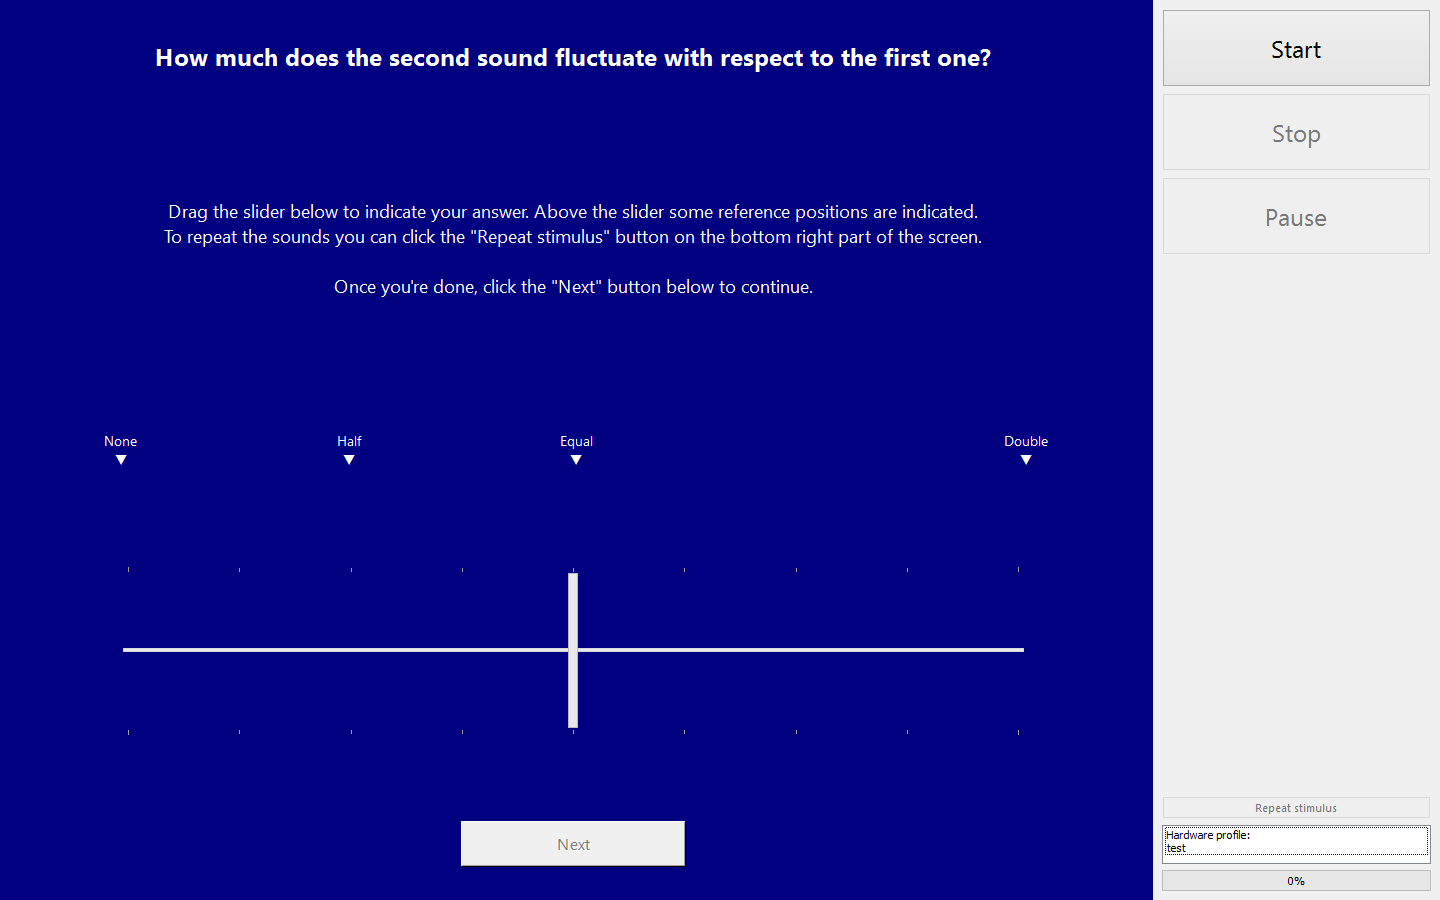
\includegraphics[width=\textwidth]{apex}
  \caption{Screenshot of the computer interface used in the final experiment
    design}
\label{fig:apex}
\end{figure}

\section{Results}

From the data obtained from the magnitude estimation procedures, it was possible
to plot the relative fluctuation strength as a function of each varying
parameter. An example of these plots is shown in \Cref{fig:fastl2007-fm}. The
actual plot pertaining the experiments will be shown in
\Cref{cha:pilot,cha:experiment}.

In order to combine the data points from the two standards, a correction factor
had to be applied to the data that used the second standard as a reference. The
correction factor was obtained taking into account the data where the second
stimulus in the pairs corresponded to the value of first standard. The
correction factor was calculated such that the median of the values that used
the second standard was the same as the median of the values that used the first
standard. An example of this can be appreciated in \Cref{fig:fastl2007-fm} panel
B, where the value of the first standard corresponds to a modulation frequency
of 4~Hz.

Finally, another correction factor was applied to all the data points, in order
to normalize the maximum mean value of the medians of the standards to 100\%.
The curve of the mean values corresponds to the black line shown in
\Cref{fig:fastl2007-fm}.

\myfigurepairlabeled%
  {fastl2007_AM-fm}
  {fastl2007_FM-fm}
  {Relative fluctuation strength as a function of modulation frequency (adapted
    from~\cite[pp.248]{Fastl2007Psychoacoustics}). The two standards had
    modulation frequencies of 4 and 0.5 Hz. The data points show the median and
    interquartile ranges per standard. The black line represents the mean values
    of the medians of each standard. Panel~A:~data for \gls{AM} tones with a
    center frequency of 1 kHz, sound pressure level of 70 dB and modulation
    depth of 40 dB. Panel~B:~data for \gls{FM} tones with a center frequency of
    1.5 kHz, sound pressure level of 70 dB and frequency deviation of 700 Hz}
  {fastl2007-fm}

\end{document}
